\section{Functional analysis}\label{ch:func}

The functional analysis of the design is described by a pair of \gls{se} tools, namely a \gls{fbs} and a \gls{ffd}. The former is an AND-tree that gives an overview of functions to be fulfilled by the system in a categorized manner; the latter expands upon this by sequencing the events. The \gls{ffd} is discussed in section \ref{sec:ffd}; the \gls{fbs} in section \ref{sec:fbs}.

\subsection{Functional Flow Diagram} \label{sec:ffd}
The \gls{ffd} is given in Figure \ref{fig:ffs}. As entry commences, the sequence and procedure for functions is to be initialized. This is done in step 1.0-1.4, which subsequently contains setting the on-board computer mode to its pre-programmed instructions for entry and conveys these instructions to the power, attitude control and thermal control subsystems. Hereafter the aeroshell is deployed - provided that the vehicle concept features a deployable aeroshell - either by mechanical means or by inflation in step 2.0-2.3. Monitoring of deployment takes place in 2.3, for example by use of measuring the pressure in the inflatable volume at selected locations for a tank-gas inflation system. In case activation is monitored to be incomplete, this is fed back and activation re-performed. The aerobraking manoeuvre then proceeds by controlling the vehicle along its trajectory, captured in function 3.1, while maintaining vehicle integrity by carrying structural and thermal loads without failure, captured in functions 3.2 and 3.3 respectively. Finally, the entry procedure is terminated at some point (described by a terminal velocity and altitude) after which \gls{taem} is activated. Hereupon other mechanisms of deceleration take over, left untreated since these are outside the scope of the mission.

\subsection{Functional Breakdown Structure} \label{sec:fbs}
The activities described in the \gls{ffd} of the previous section are categorized in the \gls{fbs}. The \gls{fbs} is given in Figure \ref{fig:fbd}.
\begin{figure}[H]
\centering
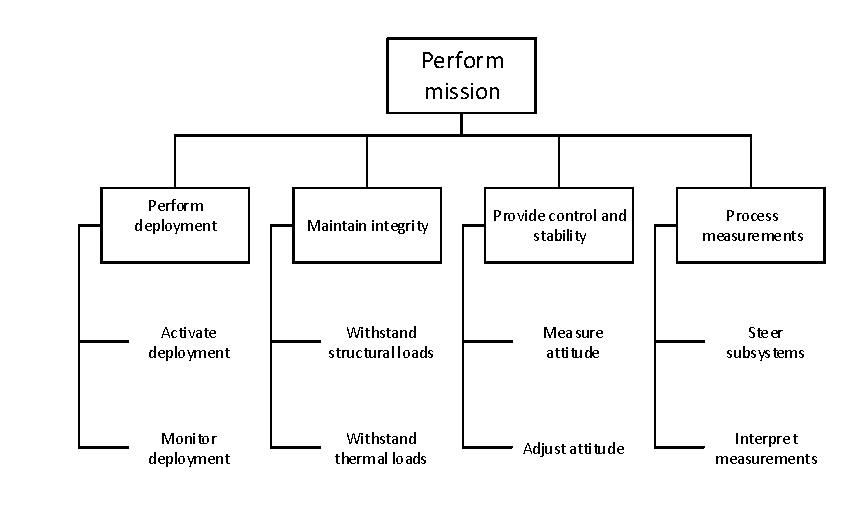
\includegraphics[width = 0.55\textwidth]{Figure/FBS.pdf}
\caption{The \gls{fbs} of the aeroshell mission}
\label{fig:fbd}
\end{figure}

\begin{figure}[H]
\hspace{-10mm}                           
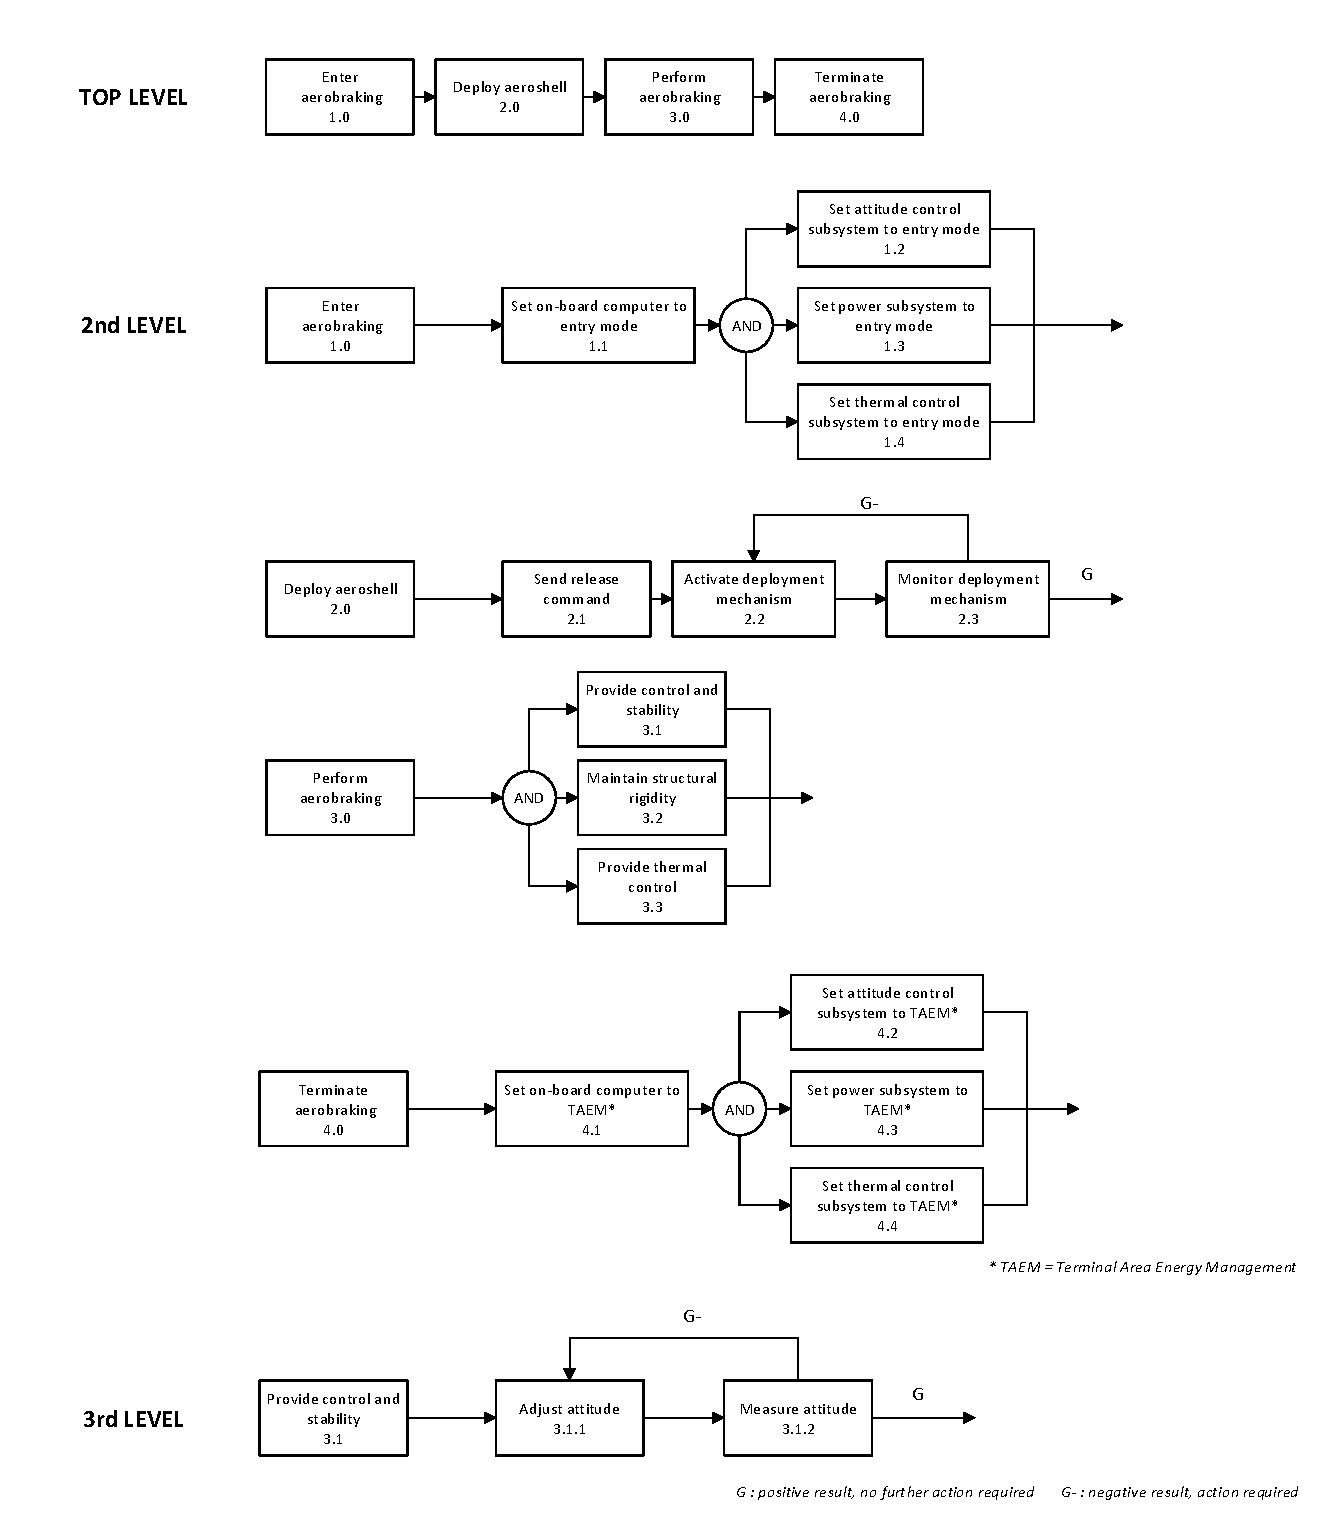
\includegraphics[width = 1.1\textwidth]{Figure/FFD.pdf}
\caption{The \gls{ffd} of the aeroshell mission}      
\label{fig:ffs}
\end{figure}